\section{Key Features through A Running Example}
\label{sec:shors}

\begin{figure}[t]
{\small
\[\hspace*{-1em}
\begin{array}{r l  l}
\textcolor{blue}{1}
&&
\{A(x) * A(y) * B \}
\quad\text{where}\;\;
A(\beta) = \beta[0..n] \mapsto \ket{\overline{0}} 
\\[0.2em]
&&
\qquad\qquad\qquad
\qquad\qquad\quad
\begin{array}{l}
B = 1 < a < N \wedge n > 0 \;\wedge
\\\qquad N < 2^n \wedge \texttt{gcd}(a,N)=1
\end{array}
\\[0.5em]
\textcolor{blue}{2}
&
&
\textcolor{teal}{
\Rightarrow
\{\dabs{\ihadh}(x[0..n]) \mapsto C * A(y) * B \}
}
\\[0.2em]
&&
\qquad\qquad\qquad
\qquad\;\;
\text{where}
\;\;
\textcolor{teal}{
C = \shad{2^n}{n}{}
}
\\[0.5em]
\textcolor{blue}{3}
& \ssassign{x}{}{\ihadh};
&
\textcolor{teal}{
\{x[0..n] \mapsto C * A(y) * B \}
}
\\[0.4em]
\textcolor{blue}{4}
&
&
\textcolor{teal}{
\Rightarrow
\{x[0..n] \mapsto C * \dabs{y\splus 1}(y[0..n]) \mapsto \ket{\overline{0}.1} * B \}
}
\\[0.4em]
\textcolor{blue}{5}
& \ssassign{y}{}{y\splus 1};
&
\textcolor{teal}{
\{x[0..n] \mapsto C * y[0..n] \mapsto \ket{\overline{0}.1} * B \}
}
\\[0.4em]
\textcolor{blue}{6}
& 
&
\textcolor{teal}{
\Rightarrow
\{ E(0) * B \}
}
\;\;
\texttt{where}\;\;
\textcolor{teal}{E(k) =}
\\[0.2em]
&&
\qquad\qquad\quad\;
\qquad
\textcolor{teal}{
\begin{array}{l}
x[0..n\,\sminus\,k] \mapsto \shad{2^{n \,\sminus\,  k}}{n \,\sminus\, k}{}\;*
\\[0.2em]
\{x[0..k],y[0..n]\} \mapsto \sch{2^k}{\frac{1}{\sqrt{2^k}}}{\tos{j}.\tos{a^{j}\;\%\;N}}
\end{array}
}
\\[0.4em]
\textcolor{blue}{7}
&\sqforh{\sint{j}{0}}{j\,\slt\, n}{x[j]}{\dplus{j}}
&
\{E(j) * B \}
\\[0.4em]
\textcolor{blue}{8}
&
\{\quad  \ssassign{y}{}{a^{2^j}y\;\%\; N}
&
\textcolor{teal}{
\{E(j\,\splus\, 1) * B \}
}
\\[0.4em]
\textcolor{blue}{9}
&
\}
&
\textcolor{teal}{
\{E(n) * B \}
}
\\[0.4em]
\textcolor{blue}{10}
&
&
\textcolor{teal}{
\Rightarrow
\{\{x[0..n],y[0..n]\} \mapsto \sch{2^{n}}{\frac{1}{\sqrt{2^{n}}}}{\tos{j}.\tos{a^{j}\;\%\;N}} * B \}
}
\\[0.4em]
\textcolor{blue}{11}
& \sexp{u}{\smea{y}}{...}
&
\textcolor{purple}{
\big{\{}
\begin{array}{l}
x[0..n] \mapsto \smch{\frac{1}{\sqrt{s}}}{s}{t\,\splus\,k p} 
\wedge
p = \texttt{ord}(a,N)
\\
\wedge\;
\texttt{nat}(u)=a^{t}\;\%\;N
\wedge
s=\texttt{rnd}(\frac{2^n}{p}) \wedge B
\end{array}
\big{\}}
}
\end{array}
\]
}
\caption{First half of the Shor's algorithm quantum part. Second half in \Cref{fig:shorqafny2}. $\snat{u}$ gets the integer number part of $u$ (mode $\mmode$). $\sord{a,N}$ gets the order of $a$ and $N$. $\srnd{r}$ rounds $r$ to the nearest integer. }
\label{fig:shorqafny}
\end{figure}

As an illustration of QNP, we implement and prove part of the Shor's algorithm in \Cref{fig:shorqafny}.
Given an integer $N$, Shor's algorithm finds its nontrivial prime factors, which has the following step: (1) randomly pick a number $1 < a < N$ and compute $k=\texttt{gcd}(a,N)$ \footnote{compute the greatest common divisor of $a$ and $N$}; (2) if $k \neq 1$, $k$ is the factor; (3) otherwise, $a$ and $N$ are coprime and we find the order $p$ of $a$ and $N$ \footnote{the order $p$ is the smallest number such that $a^p \% N = 1$}; (4) if $p$ is even and $a^{\frac{p}{2}} \neq -1 \% N$, $\texttt{gcd}(a^{\frac{p}{2}}\pm 1,N)$ are the factors, otherwise, we repeat the process. Step (2) is the quantum part of Shor's algorithm and \Cref{fig:shorqafny} and \Cref{fig:shorqafny2} show its automated proof in QNP. In \Cref{fig:shorexample}, we show the actual implementation and proof in the Qafny tool.

\begin{wrapfigure}{r}{8.2cm}
  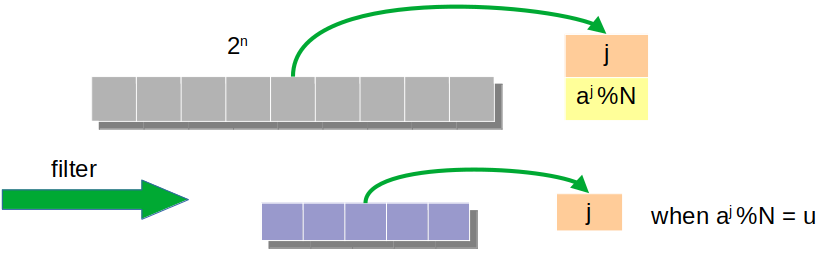
\includegraphics[width=.60\textwidth]{shorsmap}
  \caption{The array analogy of Shor's first half in \Cref{fig:shorqafny}. }
\label{fig:shorsanalog}
\end{wrapfigure}

The Shor's quantum first half in \Cref{fig:shorqafny} can be analogized as an efficient array filter operation.
The steps before line 11 (steps at line 3, 4 and 7-9) create a $2^n$-length of pairs, each of which is formed as $(j,a^j \% N)$ where $j\in [0,2^n)$. The measurement in line 11 filters the array as a new one ($x$) with all elements $j$ satisfying $a^j \% N=z$ where $z$ is a randomly picked number. Notice that modulo multiplication $f(j)=a^j\%N$ is a periodic function. All elements in $x$ satisfy $a^j \% N=z$, which means that 1) there will be a smallest $t$ such that $a^t \% N=z$, and 2) all elements can be rewritten as $j=t+kp$ and $p$ is the period of the modulo multiplication function because $a^{t+kp} \% N=z$, which is given as the post-condition on the right of line 11.
The first half implementation and correctness proof in \Cref{fig:shorqafny} exactly reflects the array analogy aspect.
One of the biggest advantage of using \qafny is that we can analogize quantum operations to classical array operations, so that we can utilize the existing automated proof infrastructure in many tools, such as Dafny.
In the Qafny implementation, verifying a quantum program usually requires only the user input of the pre-, post-, and loop invariant. For example, the proof of \Cref{fig:shorqafny} in \qafny requires none of the states marked teal, but only the conditions marked black and purple. \footnote{The purple is also not needed if we combine the Shor's first and second half algorithms together.}
Here, we step by step discuss the states, program syntax, and proofs of the aspect.

\begin{figure}[t]
{
  \small
\[\hspace*{-0.5em}
\begin{array}{l}
\textcolor{blue}{\text{Basic Terms:}}\\[0.2em]
\begin{array}{llcl llcl llcl}
\text{Nat. Num} & m, n & \in & \mathbb{N}
&
      \text{Real} & r & \in & \mathbb{R}
&
      \text{Complex Number} & z & \in & \mathbb{C}
\\
      \text{Variable} & x,y &&

 & \text{Bit} & d & ::= & 0\mid 1       
&
      \text{Bitstring} & c & \in & d^{+}      
\\
\text{Phase} & \alpha(r) & ::= & e^{2\pi i r}
\\
\end{array}
\\[1em]
\textcolor{blue}{\text{Modes, Kinds, Types, and Classical/Quantum Values:}}\\[0.2em]
\begin{array}{llclll} 
      \text{Mode} & g & ::= & \cmode  \mid \mmode\\
      \text{Classical Value} & v & ::= & n \mid (r,n)\\
      \text{Full Mode (Kind)} & \overline{g} & ::= & g \mid \qmode{n} \\
      \text{Quantum Type} & \tau & ::= & \tnort &\mid \thadt & \mid \tcht \\
      \text{Quantum Value} & q & ::= & \ket{c} & \mid \shad{2^n}{n}{\alpha(r_j)} &\mid \sch{m}{z_j}{c_j \,\beta_j} \\
    \end{array}
\\[1em]
\textcolor{blue}{\text{Quantum Sessions, Environment, and States}}\\[0.2em]
\begin{array}{llclcl} 
      \text{Range} & l & ::= & x[n..m] \\
      \text{Session} & \lambda & ::= & \overline{x[n..m]} & \text{by} & \uplus \\
      \text{Type Environment} & \sigma & ::= & \overline{\lambda : \tau } & \text{by} & \cup \\
      \text{Quantum State} & \varphi & ::= & \overline{ \lambda : q } & \text{by} & \cup \\
    \end{array}
\end{array}
  \]
}
  \caption{\qafny element syntax. Each range $x[n..m]$ in a session $\overline{x[n..m]}$ represents the number range $[n,m)$ in a qubit array $x$. Sessions are finite lists, while type environments and states are finite sets. the operations after "by" refer to the concatenation operations for session, type environments and quantum states. }
  \label{fig:qafny-state}
\end{figure}

\myparagraph{Classical and Quantum States}
On the right of \Cref{fig:shorqafny} line 1, it is the the pre-condition of the program, which describes two quantum arrays; both are initialized to be $n$-qubit of bits $0$ (as $\overline{0}$), represented as predicates $A(x)$ and $A(y)$, and other restrictions for integers $a$ and $N$ represented as predicate $B$.
In Qafny, there are three kinds of values, two of which are classical ones represented by the two modes: $\cmode$ and $\mmode$ in \Cref{fig:qafny-state}. The former represents classical values, represented as a natural number $n$, that do not intervene with quantum measurements and are evaluated in the compilation time, the latter represents values, represented as a pair $(r,n)$, produced from a quantum measurement. The real number $r$ is a characteristic representing the theoretical probability of the measurement resulting in the natural number value $n$. In \Cref{fig:shorqafny}, $a$ and $N$ are $\cmode$-mode values and $u$ is a $\mmode$ value so that we can use function $\texttt{nat}$ to produce its natural number part. Quantum values are defined in the units of qubit arrays that represent potentially entangled qubit clusters and are represented as kind $\qmode{n}$, where $n$ is the array size. \qafny represents qubit arrays as \emph{sessions} ($\lambda$), which consist of different \emph{disjoint ranges}, each of which describes an array fragment $x[n..m]$, where $x$ is a variable representing a qubit array piece, named a qubit group, initialized by an \texttt{init} statement, and $[n..m]$ represents the array fragment from position $n$ to $m$ (exclusive) in group $x$.
For simplicity, we assume that there are no aliasing array piece variables in this paper, i.e., two distinct variables represent disjoint array pieces. For example, $\{\{x[0..n],y[0..n]\}$ in \Cref{fig:shorqafny} line 10 represents a $2n$ qubit array containing two disjoint pieces $x[0..n]$ and $y[0..n]$ referring to the ranges $[0,n)$ in groups $x$ and $y$, respectively.
We also abbreviate a singleton session $\{x[n..m]\}$ as a range $x[n..m]$.

Each length-$n$ session is associated to a quantum state with the same length that can be one of the three forms ($q$ in \Cref{fig:qafny-state}) that are corresponding to three different types ($\tau$ in \Cref{fig:qafny-state}). 
A $\tcht$-type session has state form $\sch{m}{z_j}{c_j\,\beta_j}$, which is the most general quantum state representation and is designed as an analogy to classical arrays in the sense that each quantum state basis is viewed as an individual array element that does not Intervene with other elements.
For example, In \Cref{fig:shorqafny} line 10, session $\{\{x[0..n],y[0..n]\}$ has state $\sch{2^{n}}{\frac{1}{\sqrt{2^{n}}}}{\tos{j}.\tos{a^{j}\;\%\;N}}$, represented as a $2^n$ entanglement array, whose element is a triple of an amplitude $\frac{1}{\sqrt{2^{n}}}$, a basis $\tos{j}.\tos{a^{j}\;\%\;N}$ \footnote{$\tos{j}.\tos{a^{j}\;\%\;N}$ can be split into $\tos{j}$ and $\tos{a^{j}\;\%\;N}$ -- both are $n$-length bitstrings and the the basis states for the $n$-length group $x[0..n]$ and $y[0..n]$, respectively.}, and an empty $\beta_j$ term. The state is represented in \qafny as an array of the form: $\frac{1}{\sqrt{2^{n}}}\ket{\tos{0}.\tos{a^{0}\;\%\;N}}+...+\frac{1}{\sqrt{2^{n}}}\ket{\tos{n-1}.\tos{a^{n-1}\;\%\;N}}$; thus, applying any quantum unitary operation on the state results in applying the operation on individual basis term $\frac{1}{\sqrt{2^{j}}}\ket{\tos{j}.\tos{a^{j}\;\%\;N}}$ in the state, which indicates that a unitary operation on a quantum state is analogized to an array map function.

The state representation of the other two types$ \tnort$ and $\thadt$ is an array of qubits rather than a basis state in the $\tcht$ type state.
A $\tnort$ type state has the form $\ket{c}$ which is a qubit array, each element of which is $0$ or $1$. The $A(x)$ predicate in \Cref{fig:shorqafny} line 1 means that an $n$-size session $x[0..n]$ has $\tnort$ type state $\ket{\overline{0}}$ with $n$ qubits and all are bit $0$. A $\thadt$ type state has the form $\shad{2^n}{n}{\alpha(r_j)}$, which represents an $n$-length array of qubits that are in superposition but not entangled. We represent the state based on qubit elements for these two types because the split and join of a session is as simple as the split and join of an array, while the join of two $\tcht$ type sessions are computing the Cartesian product and the split of a $\tcht$ type state is disentanglement, a very hard problem.
In many quantum algorithms, the entangled qubit establishment is to add a single superposition qubit to an existing $\tcht$ type session.
For example, in the loop body in line 8, each iteration grows the entanglement session $\{x[0..j],y[0..n]\}$ to $\{x[0..j\,\splus\,1],y[0..n]\}$ by adding a $\thadt$ type qubit $\{x[j\,\sminus\,1..j]\}$ that is split from the \thadt type session $\{x[0..j]\}$.
In this procedure, the elements $\tcht$ state are doubled, which will be explained shortly.

\begin{figure}[t]
{
  \small
  \[\begin{array}{llcl} 
      \text{\oqasm Expr} & \mu\\
      \text{Parameter} & l & ::= & x \mid x[a] \\
      \text{Arith Expr} & a & ::= & x \mid v \mid a + a \mid a * a \mid ... \\
      \text{Bool Expr} & b & ::= & x[a] \mid (a = a) @ x[a] \mid (a < a) @ x[a] \mid ... \\
      \text{Predicate} & P & ::= & a = a \mid a < a \mid \lambda \mapsto q \mid P \wedge P \mid P * P \mid ... \\
      \text{Gate Expr} & op & ::= & \texttt{H} \mid \iqft[\lbrack -1 \rbrack]{}{} \\
      \text{C/M Moded Expr}& e & ::= & a \mid \sinit{a} \mid \smea{y} \mid \textcolor{red}{\sret{y,(r,n)}} \\
      \text{Statement} & s & ::= & \sskip \mid \sexp{x}{e}{s} \mid  \ssassign{l}{}{op} \mid \ssassign{\lambda}{}{\mu} 
                                 \mid \ssassign{l}{}{\sdis}
                                 \\ & & \mid & \sseq{s}{s} \mid \sifq{b}{s} \mid
                                     \sqwhile{j}{a_1}{a_2}{b}{s}
    \end{array}
  \]
}
  \caption{Core \qafny syntax. \oqasm is in \Cref{sec:vqir}. For an operator \texttt{OP}, $\texttt{OP}^{\lbrack -1 \rbrack}$ indicates that the operator has a built-in inverse available. Arithmetic expressions in $e$ are only used for classical operations, while Boolean expressions are used for both classical and quantum operations. $x[a]$ represents the $a$-th element in the qubit array $x$, while a quantum variable $x$ represents the qubit group $x[0..n]$ and $n$ is the length of $x$. }
  \label{fig:vqimp}
\end{figure}

\myparagraph{Language Syntax} One of the key \qafny design principles is to allow programmers think of quantum programs as sequences of functional operations that are analogized to array map functions, instead of dealing with quantum circuit gates in many other languages.
For example, line 3 in \Cref{fig:shorqafny}, we prepare a state by applying a series of \texttt{H} to each qubit in group $x$. In an iteration in line 8, for the session $\{\{x[0..n],y[0..n]\}$ having $\tcht$ type, the operation first selects the basis states where the $x[j]$ qubit basis being $1$, then applies the modulo multiplication ${a^{2^j}y\;\%\; N}$ only to these basis states.
\Cref{fig:vqimp} shows the \qafny syntax.
A program consists of a sequence of C-like statements $s$ that end at a SKIP operation $\sskip$.
The let operation ($\sexp{x}{e}{s}$) in the first row introduces a new variable $x$ with its initial value defined $e$ and used in $s$. If $e$ is an arithmetic expression ($a$), it introduces a $\cmode$ or $\mmode$ classical variable. For simplicity, we assume that $\mmode$ arithmetic operations manipulates the \texttt{nat} number parts, so that $(r,n_1)+n_2=(r,n_1+n_2)$; and we only interacts a $\mmode$ value with a $\cmode$ one in an arithmetic operation, i.e., the $(r_1,n_1)+(r_2,n_2)$ is disallowed in \qafny. $\sexp{x}{\sinit{a}}{s}$ initializes an $a$-length qubit group named $x$ with the value $\ket{\overline{0}}$ ($a$ number of bit $0$) and is used in statement $s$, while $\sexp{x}{\smea{y}}{s}$ measures qubit group $y$, stores the result in $\mmode$-mode variable $x$, and is used in $s$.
The measurement semantic definition relies on a ghost expression $\texttt{ret}$, and it turns $\smea{y}$ to $\sret{y,(r,n)}$, which does not appear in a \qafny source program but appears during semantic evaluation, and it records the intermediate measurement result of group $y$ as $(r,n)$.

The last three operations in first row are the quantum data-flow operations.
$\ssassign{l}{}{op}$ is a quantum state preparation operation that prepares superposition of quantum qubits $l$ through Hadamard gates $\texttt{H}$ or $\texttt{QFT}$ gates. It is also used to transform quantum qubit states by a $\texttt{QFT}^{-1}$ gate in the end of the quantum phase estimation algorithm. 
We only permit $op$ to be state preparation gates such as \texttt{H} and $\iqft[\lbrack -1 \rbrack]{}{}$ gates.
The other gate applications are done through $\ssassign{\lambda}{}{\mu}$ that performs quantum oracle computation $\mu$ on each basis state of a $\tcht$ type session $\lambda$, such as quantum arithmetic operation. While let operation only performs classical arithmetic computation, quantum oracle arithmetic operation is performed through \oqasm expressions \cite{oracleoopsla} (also in \Cref{sec:vqir}), which can be used to define almost all reversible arithmetic operations such as the ones in \Cref{fig:vqimp}. 
For example, the Shor's algorithm implementation in \Cref{fig:shorqafny} utilizes the addition (line 5) and modulo multiplication (line 8) on qubit group $y$, which can be expressed as an \oqasm circuit.
$\ssassign{l}{}{\sdis}$ is a quantum diffusion operation applying on the parameter $l$, where $l$ may be part of a session.
The main functionality is to increase and average the occurrence likelihood of some quantum bases in a quantum state. Details are in \Cref{sec:vqir}.

The second row of statements in \Cref{fig:vqimp} are control-flow operations.
$\sseq{s_1}{s_2}$ is a sequential operation.
$\sifq{b}{s}$ is a classical or quantum conditional depending on if $b$ contains quantum parameter.
%Every quantum parameter $l$ appearing in $b$ must not appear in $s$.
%In the \qafny type system, we define a \texttt{well\_formed} predicate to check such property.
If $b$ is quantum, it must be reversible as quantum gate applications are essentially unitary matrix operations.
The reversibility requires that a Boolean equality and inequality expression to be written as $(a_1 = a_2) @ x[a]$ and $(a_1 < a_2) @ x[a]$, respectively; where an additional bit $x[a]$ is required to hold the result of computing $a_1=a_2$ or $a_1<a_2$.
$\sqwhile{j}{a_1}{a_2}{b}{s}$ is a possibly quantum for-loop depending on if $b$ contains quantum parameters.
A classical variable $j$ is introduced and it is initialized as the lower bound $a_1$, increments in each loop step defined by $\dplus{j}$, and ends at the upper bound $a_2$.
For example, line 7-9 in \Cref{fig:shorqafny} uses a for-loop to repeatably entangle the $x[j]$ qubit with the entangled qubit session $\{x[0..j],y[0..n]\}$ with the application of the modulo multiplication at line 8.
In \qafny implementation, $\dplus{j}$ and $j<a_2$ can be arbitrary monotonic increment and comparison functions.
For simplicity, we restrict the two to be $\dplus{j}$ and $j<a_2$ in this paper.

\myparagraph{Proofs in \qafny} QNP intends to create a proof system that utilizes classical automated reasoning infrastructure in analyzing quantum programs. As we introduced above, quantum operations can be analogized to classical array map functions.
Thus, the prototype of designing the QNP proof system is the array application rule in classical Hoare Logic \cite{Gordon12backgroundreading}, written as:

{\small
\begin{center}
$\{P[\wp(\lambda)/\lambda]\} \ssassign{\lambda}{}{\wp} \{P\}$
\end{center}
}

We analogize array variable as the quantum state sessions that are represented arrays here.
$\wp(\lambda)$ is the result of applying an operation $\wp$ to every element in $\lambda$. 
For example, in \Cref{fig:shorqafny} line 3, the post-condition of apply the $\texttt{H}$ gate is $x[0..n] \mapsto C * A(y) * B$, so that the pre-condition in line 2 is $\dabs{\ihadh}(x[0..n]) \mapsto C * A(y) * B$, by replacing $x[0..n]$ with $\dabs{\ihadh}(x[0..n])$.
The state $A(x)\equiv x[0..n]\mapsto \ket{\overline{0}}$ in line 1 can be rewritten to $\dabs{\ihadh}(x[0..n]) \mapsto C$, because if we apply $\dabs{\ihadh}$ on the both side, it becomes:

{\small
\begin{center}
 $\dabs{\ihadh}(x[0..n]) \mapsto \dabs{\ihadh}(\ket{\overline{0}}) = \shad{2^n}{n}{} = C
\qquad 
\texttt{where}
\;\;
\dabs{\ihadh}(\ket{0})= \frac{1}{\sqrt{2}}(\ket{0}+\ket{1})
$
\end{center}
}

The right hand side formula is a typical superposition state preparation by a Hadamard gate in quantum computation.
In \qafny, we are using the separating conjunction operation $*$ from separation logic \cite{separationlogic}, where $\varphi \cup \varphi' \models P * Q$ iff $\varphi \bot \varphi'$ and $\varphi \models P$ and $\varphi' \models Q$. Here, $\varphi$ and $\varphi'$ are finite quantum states mapping from sessions to the three forms above.

In mapping \qafny rules to classical array proof rules, there are three subtleties. First, sessions are both indicators, which are viewed as array structures that record qubit positions, for entangled qubit groups; as well as variables, which are viewed as names, representing qubit states in pre- and post-conditions.
In preserving the two session roles, we design a type system in \Cref{sec:vqir} 
to track transitions of sessions and require that 
a well-formed pre-condition only mentions the sessions defined in a given type environment.
Second, we also define equational properties, representing the permutation symmetries of quantum states, for 
sessions and quantum states mapping from sessions to the three forms above.
This permits the use of ideal quantum state form in proving a statement.
For example, in \Cref{fig:shorqafny} line 10, the session $\{\{x[0..n],y[0..n]\}$ has the state $\sch{2^{n}}{\frac{1}{\sqrt{2^{n}}}}{\tos{j}.\tos{a^{j}\;\%\;N}}$, which can also be equivalently formulated as a session $\{\{y[0..n],x[0..n]\}$ having the state 
$\sch{2^{n}}{\frac{1}{\sqrt{2^{n}}}}{\tos{a^{j}\;\%\;N}.\tos{j}}$ by switching the $x$ and $y$ positions. Details are in \Cref{sec:state}.

Third, line 7-9 describes the transition for a for-loop based on a series of quantum conditionals.
In each iteration, a $\thadt$ type qubit $x[j]$ is joined into the entangled session $\{x[0..j],y[0..n]\}$, 
so that the session is extended to $\{x[0..\snext{j}],y[0..n]\}$ and the basis state number is doubled.
Then, the conditional body modulo multiplication in line 8 is applied to exactly half of the basis states whose $x[j]$ position's bit value is $1$, while the others are preserved to be the same.
There are two mysterious points in the above scenario.
The first one is the quantum state split and join operations that can be captured by additional equational properties in \Cref{sec:state}.
The second point is the proof rule for a quantum conditional that represents the partial map behavior where operations in the conditional body are only applied to some of the basis states. Details are in \Cref{sec:typesystem}.

Fourth, line 11 is a partial measurement operation. Given a quantum state $\varphi$, a measurement is the only operation that modifies $\varphi$'s domain and it cannot be placed inside a quantum conditional; otherwise, the system leaks quantum information during a quantum computation, a violation of a quantum information principle. More details are in \Cref{sec:semantics}.
